\chapter{Тестирование}

Проведем несколько тестов на правильность решения задачи оптимизации. Тестирование будем проводить следующим образом: будем брать множество точек, проверить правильность решения задачи минимизации которой интуитивно не вызывает особого труда. Иными словами, будем брать $m$ точек для задачи, которые или удовлетворяют функции, или находятся в непосредственной близости к множеству точек, удовлетворяющим значениям функции.
Искомые функции будут иметь следующий вид:
\begin{itemize}
	\item для линейной функции в N-мерном пространства в качестве примера рассмотрим $F(\vec{x}) = 1 + x_1 + x_2$;
	\item для полинома -- $P(x) = 1 + 3x + 3x^2 - x^3$;
	\item для кусочно-линейной функции - $f(x) = -1 + |x+1|-|x|+|x+1|$;
	\item для сглаживающего сплайна возьмем пример из учебника "Метод конечных элементов для решения скалярных и векторных задач" на странице 214.
\end{itemize}

Искомые функции изображены на рисунках \ref{fig:LineN} -- \ref{fig:Spline}.

\begin{figure}
	\centering
	\vspace*{0.7cm}
	\includegraphics[width=0.5\linewidth]{images/"Flat1".png}
	\caption{Линейная функция в 3-х мерном пространстве}
	\label{fig:LineN}
\end{figure}


\begin{figure}
	\centering
	\vspace*{0.7cm}
	\includegraphics[width=0.5\linewidth]{images/"Flat2".png}
	\caption{Линейная функция в 3-х мерном пространстве (вид сверху)}
	\label{fig:LineN1}
\end{figure}


\begin{figure}
	\centering
	\vspace*{0.7cm}
	\includegraphics[width=0.5\linewidth]{images/"Flat3".png}
	\caption{Линейная функция в 3-х мерном пространстве (вид сбоку)}
	\label{fig:LineN2}
\end{figure}


\begin{figure}
	\centering
	\vspace*{0.7cm}
	\includegraphics[width=0.5\linewidth]{images/"Polynomial".png}
	\caption{Полиномиальная функция}
	\label{fig:Polynomial}
\end{figure}

\begin{figure}
\centering
\vspace*{0.7cm}
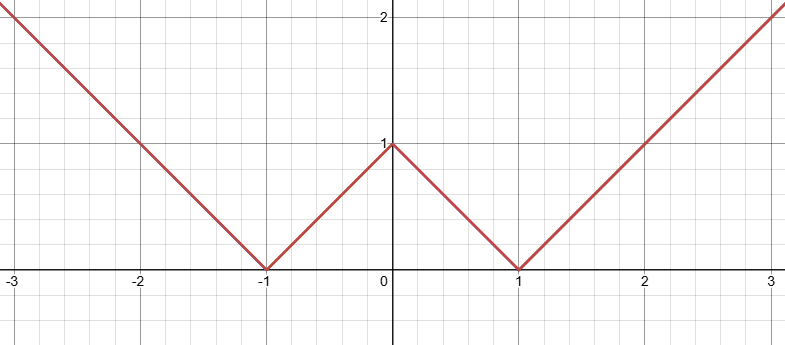
\includegraphics[width=0.6\linewidth]{images/PW.png}
\caption{Кусочно-линейная функция}
\label{fig:PW}
\end{figure}

\begin{figure}
\centering
\vspace*{0.7cm}
\includegraphics[width=0.5\linewidth]{images/"Spline".png}
\caption{Сглаживающий сплайн}
\label{fig:Spline}
\end{figure}

Коэффициенты решения для сглаживающего сплайна выглядит следующим образом: $q = \left[2.5, -0.0117, 2.48, -0.0673, 0.0488, -3.35\right]$.

Тестовые входные данные с координатами точек хранятся в директории \text{/SciDevOOP/bin/Resources}. Содержимое этих файлов представлено в таблице \ref{tab:testData}.

\begin{table}
	\caption{Содержимое файлов с входными данными}
	\centering
	\small
	\begin{tabularx}{1.0\textwidth}{| >{\raggedright\arraybackslash}X | >{\raggedright\arraybackslash}X | >{\raggedright\arraybackslash}X | >{\raggedright\arraybackslash}X |}
		\hline
		\centering{Линейная 3-х мерная}  & \centering{Полином} & \centering{Кусочно-постоянная} & \centering{Сплайн} \tabularnewline \hline    
			\text{7}\newline
			\text{0 0 1} \newline
			\text{1 0 2} \newline
			\text{0 1 2} \newline
			\text{1 1 3} \newline
			\text{0,5 0 1,5} \newline
			\text{0 0,5 1,5} \newline
			\text{0,5 0,5 2} \newline  & 
			\text{15} \newline
			\text{-2,5 27,875} \newline
			\text{-2 15} \newline
			\text{-1,5 6,625} \newline
			\text{-1 2} \newline
			\text{-0,5 0,375} \newline
			\text{0 1} \newline
			\text{0,5 3,125} \newline
			\text{1 6} \newline
			\text{1,5 8,875} \newline
			\text{2 11} \newline
			\text{2,5 11,625} \newline
			\text{3 10} \newline
			\text{3,5 5,375} \newline
			\text{4 -3} \newline
			\text{4,5 -15,87} \newline & 
			\text{9} \newline
			\text{-2 1} \newline
			\text{-1,5 0,5} \newline
			\text{-1 0} \newline
			\text{-0,5 0,5} \newline
			\text{0 1} \newline
			\text{0,5 0,5} \newline
			\text{1 0} \newline
			\text{1,5 0,5} \newline
			\text{2 1} & 
			\text{11} \newline
			\text{0,0 2,5} \newline
			\text{0,5 2,5} \newline
			\text{1,1 2,5} \newline
			\text{1,5 2,5} \newline
			\text{2,0 2,5} \newline
			\text{2,5 2,5} \newline
			\text{3,0 2,5} \newline
			\text{4,0 2,3} \newline
			\text{4,5 1,2} \newline
			\text{4,8 0,8} \newline
			\text{5,0 0,0} \newline \tabularnewline \hline    
	\end{tabularx}
	\label{tab:testData}
\end{table}

\section{Тестирование метода имитации отжига}


\begin{table}
	\caption{Тестирование 3-х мерной линейной функции $P(\vec{x}) = 1 + x_1 + x_2$.}
	\centering
	\small
	\begin{tabularx}{1.0\textwidth}{| >{\centering\arraybackslash}X | >{\raggedright\arraybackslash}X | >{\raggedright\arraybackslash}X |}
		\hline
		\centering{Начальные параметры}  & \centering{Функционал} & \centering{Средний результат из 10 решений} \tabularnewline \hline    
		
		\multirow{4}{*}{\centering{0.89, 0.5, 0.5}} & $L_1$ & \centering{9.985284E-001, 1.000726E+000, 1.001621E+000} \tabularnewline \cline{2-3}
		
		& $L_2$ & \centering{1.003186E+000, 9.977719E-001, 9.964673E-001} \tabularnewline \cline{2-3}
		
		& $L_{\inf}$ & \centering{9.988302E-001, 1.003419E+000, 9.985865E-001} \tabularnewline \cline{2-3}
		
		& Интеграл & \centering{0.00000000E+000; 0.00000000E+000; 0.00000000E+000} \tabularnewline \hline
	\end{tabularx}
	\label{tab:testLineN1}
\end{table}


\begin{table}
	\caption{Тестирование кусочно-линейной функции $f(x) = -1 + |x + 1| + |x| + |x - 1|$.}
	\centering
	\small
	\begin{tabularx}{1.0\textwidth}{| >{\centering\arraybackslash}X | >{\centering\arraybackslash}X | >{\centering\arraybackslash}X |}
		\hline
		Начальные параметры  & Функционал & Средний результат из 10 решений \tabularnewline \hline    
		
		\multirow{4}{*}{\makecell{0.8, 0.7, 0.9, -0.78\\ -1.87, -1.0, 0.0, 1.0}}  & $L_1$ & 2.864295E-002, -1.044582E+000, 9.740291E-001, -9.856934E-001, 1.033343E+000 \tabularnewline \cline{2-3}
		
		& $L_2$ & 9.581629E-004, -1.100468E+000, 1.060370E+000, -1.067029E+000, 1.081162E+000 \tabularnewline \cline{2-3}
		
		& $L_{\inf}$ & -1.847915E-002, -9.562990E-001, 9.900883E-001, -9.708578E-001, 9.495355E-001 \tabularnewline \cline{2-3}
		
		& Интеграл & 0.00000000E+000; 0.00000000E+000; 0.00000000E+000 \tabularnewline \hline
	\end{tabularx}
	\label{tab:testPW1}
\end{table}

\begin{table}
	\caption{Тестирование полиномиальной функции $P(x) = 1 + 3x + 3x^2 - x^3$.}
	\centering
	\small
	\begin{tabularx}{1.0\textwidth}{| >{\centering\arraybackslash}X | >{\raggedright\arraybackslash}X | >{\raggedright\arraybackslash}X |}
		\hline
		\centering{Начальные параметры}  & \centering{Функционал} & \centering{Средний результат из 10 решений} \tabularnewline \hline    
		
		\multirow{4}{*}{\centering{0.8, 0.7, 0.9, -0.28}} & $L_1$ & \centering{9.760448E-001, 3.056967E+000, 3.025434E+000, -1.009347E+000} \tabularnewline \cline{2-3}
		
		& $L_2$ & \centering{1.043514E+000, 2.921941E+000, 3.004910E+000, -9.983161E-001} \tabularnewline \cline{2-3}
		
		& $L_{\inf}$ & \centering{1.127008E+000, 3.080072E+000, 3.011509E+000, -1.007120E+000} \tabularnewline \cline{2-3}
		
		& Интеграл & \centering{0.00000000E+000; 0.00000000E+000; 0.00000000E+000} \tabularnewline \hline
	\end{tabularx}
	\label{tab:testPolynomial1}
\end{table}

\begin{table}
	\caption{Тестирование сплайна $q = \left[2.5, -0.0117, 2.48, -0.0673, 0.0488, -3.35\right]$.}
	\centering
	\small
	\begin{tabularx}{1.0\textwidth}{| >{\centering\arraybackslash}X | >{\centering\arraybackslash}X | >{\centering\arraybackslash}X |}
		\hline
		Начальные параметры & Функционал & Средний результат из 10 решений \tabularnewline \hline    
		
		\multirow{4}{*}{\makecell[c]{0.5, 0.0, 1.47, \\ -0.78, 1.88, -0.35, \\ 0.0, 2.0, 5.0}} & $L_1$ & \centering{2.572843E+000, -3.772355E-001, 2.486581E+000, -2.242274E-001, 2.995627E-002, -3.614091E+000} \tabularnewline \cline{2-3}
		
		& $L_2$ & \centering{2.500145E+000, -1.446680E-001, 2.490407E+000, -9.458615E-002, 2.340403E-002, -3.365737E+000} \tabularnewline \cline{2-3}
		
		& $L_{\inf}$ & \centering{2.399551E+000, 1.817553E-001, 2.490943E+000, -6.092797E-002, 2.510118E-002, -3.336969E+000} \tabularnewline \cline{2-3}
		
		& Интеграл & 0.00000000E+000; 0.00000000E+000; 0.00000000E+000 \tabularnewline \hline
	\end{tabularx}
	\label{tab:testSpline1}
\end{table}

\section{Тестирование метода сопряжённых градиентов}
\begin{table}
	\caption{Тестирование 3-х мерной линейной функции $P(\vec{x}) = 1 + x_1 + x_2$.}
	\centering
	\small
	\begin{tabularx}{1.0\textwidth}{| >{\centering\arraybackslash}X | >{\centering\arraybackslash}X | >{\raggedright\arraybackslash}X |}
		\hline
		\centering{Начальные параметры}  & \centering{Функционал} & \centering{Результат} \tabularnewline \hline    
		
		\multirow{2}{*}{\centering{-1.5, 0.1, 1.0}} & $L_1$ & \centering{1.000000E+000, 1.000000E+000, 1.000000E+000} \tabularnewline \cline{2-3}
		
		& $L_2$ & \centering{1.000000E+000, 9.999999E-001, 9.999998E-001} \tabularnewline \hline
	\end{tabularx}
	\label{tab:testLineN2}
\end{table}

\begin{table}
	\caption{Тестирование кусочно-линейной функции $f(x) = -1 + |x + 1| + |x| + |x - 1|$.}
	\centering
	\small
	\begin{tabularx}{1.0\textwidth}{| >{\centering\arraybackslash}X | >{\centering\arraybackslash}X | >{\raggedright\arraybackslash}X |}
		\hline
		\centering{Начальные параметры}  & \centering{Функционал} & \centering{Результат} \tabularnewline \hline    
		
		\multirow{4}{*}{\makecell[c]{0.7, 0.4, 0.1, 0.1, \\ 0.2, -1.0, 0.0, 1.0}} & $L_1$ & \centering{7.003582E-002, -8.814619E-001, 8.784511E-001, -9.392526E-001, 9.824676E-001} \tabularnewline \cline{2-3}
		
		& $L_2$ & \centering{2,217045E-01
			7,360733E-02
			-7,448983E-02
			7,741301E-02
			3,293158E-01} \tabularnewline \hline
	\end{tabularx}
	\label{tab:testPW2}
\end{table}


\section{Тестирование метода Левенберга — Марквардта}

\begin{table}
	\caption{Тестирование 3-х мерной линейной функции $P(\vec{x}) = 1 + x_1 + x_2$.}
	\centering
	\small
	\begin{tabularx}{1.0\textwidth}{| >{\centering\arraybackslash}X | >{\centering\arraybackslash}X | >{\raggedright\arraybackslash}X |}
		\hline
		\centering{Начальные параметры}  & \centering{Функционал} & \centering{Результат} \tabularnewline \hline    
		
		\multirow{4}{*}{\centering{-1.0, 0.1, 2.0}} & $L_2$ & \centering{1.000000E+000, 1.000000E+000, 1.000000E+000} \tabularnewline \hline
	\end{tabularx}
	\label{tab:testLineN3}
\end{table}

\begin{table}
	\caption{Тестирование кусочно-линейной функции $f(x) = -1 + |x + 1| + |x| + |x - 1|$.}
	\centering
	\small
	\begin{tabularx}{1.0\textwidth}{| >{\centering\arraybackslash}X | >{\centering\arraybackslash}X | >{\raggedright\arraybackslash}X |}
		\hline
		\centering{Начальные параметры}  & \centering{Функционал} & \centering{Результат} \tabularnewline \hline    
		
		\multirow{4}{*}{\makecell[c]{0.7, 0.4, 0.1, 0.1, \\ 0.2, -1.0, 0.0, 1.0}} & $L_2$ & \centering{9.585372E-15, -1.000000E+00, 1.000000E+00, -1.000000E+00, 1.000000E+00} \tabularnewline \hline
		
	\end{tabularx}
	\label{tab:testPW3}
\end{table}